\chapter{Arquitetura e Implementação}
\label{chap:arquitetura-implementacao}
O ponto de entrada do sistema é o \texttt{SchedulingEngine}, definido em
\texttt{src/main.py}. Este componente centraliza a inicialização das
configurações, instancia os módulos necessários e determina do fluxo de
execução. 

Esta camada não implementa diretamente a lógica de formulação, decomposição ou
resolução. O seu papel é orquestrar os componentes da arquitetura, mantendo cada
responsabilidade encapsulada no respetivo módulo.

A partir daqui, a arquitetura foi desenhada com dois objetivos principais: modularidade e separação de
responsabilidades. A modularidade permite trocar
a origem dos dados, comparar estratégias de resolução e introduzir novas formas
de decomposição sem alterar toda a pipeline. Já as responsabilidades foram distribuídas por
quatro componentes: captura de processos, formulação \acs{QUBO},
resolução por \textit{solvers} e validação/análise. 

\begin{figure}[H]
\centering
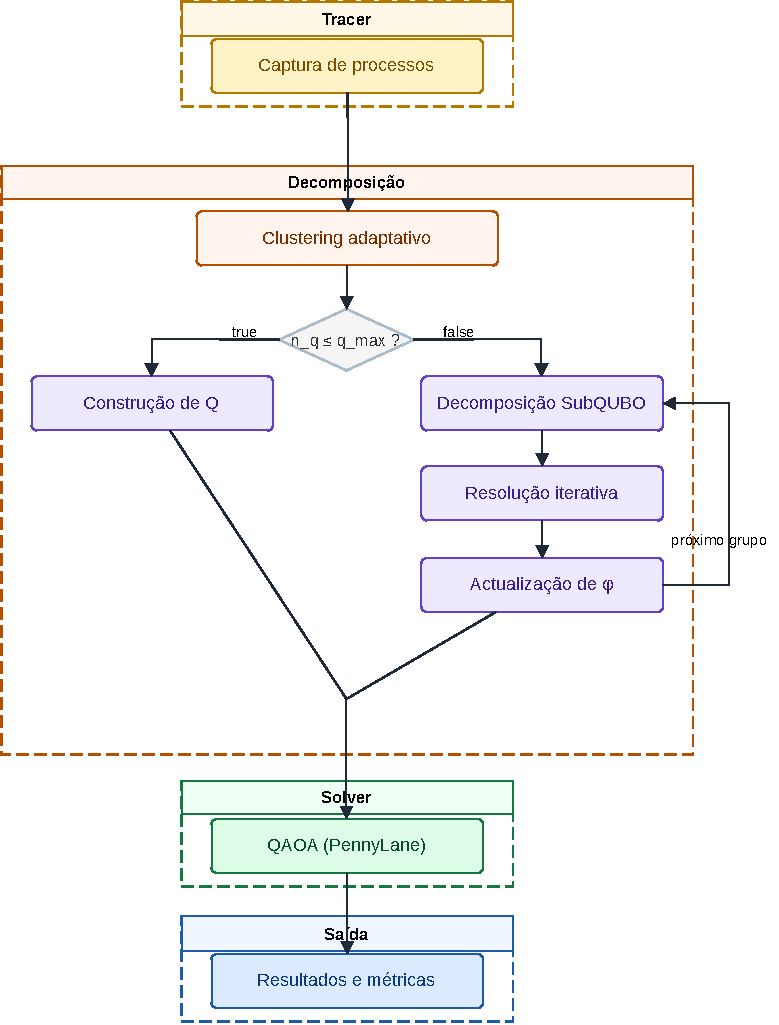
\includegraphics[width=\textwidth,height=0.47\textheight,keepaspectratio]{images/diagrams/visao-geral-arquitetura/visao-geral-arquitetura.pdf}
\caption{Visão geral do fluxo da arquitetura.}
\label{fig:arquitetura-visao-geral}
\end{figure}

A Figura~\ref{fig:arquitetura-visao-geral} ilustra o fluxo completo da
arquitetura, desde a aquisição dos processos até à produção dos resultados.

O fluxo de execução começa pelo Tracer. O objectivo desta camada é produzir
uma descrição dos processos a escalonar (cargas de \acs{CPU}, memória utilizada
e núcleo atual), que serve de base a todo o resto da pipeline. Antes de poder
ser entregue ao \textit{solver}, essa descrição tem de ser traduzida para uma
representação matemática que o algoritmo de optimização compreenda: uma
instância \acs{QUBO}. A zona de decomposição é responsável por essa tradução e,
consoante a dimensão do problema, segue um de dois caminhos:

\begin{itemize}
    \item quando $n_q \leq q_{max}$, é construída uma única matriz $Q$ e a
    instância é resolvida directamente pelo \textit{solver};
    \item quando $n_q > q_{max}$, os processos são primeiro agrupados em
    \textit{bundles} e o problema é decomposto em \textit{sub-QUBOs}
\end{itemize}

Independentemente do ramo seguido, o resultado é uma ou mais instâncias
\acs{QUBO} entregues ao \textit{solver}. A solução obtida é depois validada,
descodificada em atribuições processo--núcleo e convertida em métricas e
ficheiros de saída.

\section{Da Visão Geral à Implementação}
\label{sec:arquitetura-implementacao}

Agora que temos uma visão geral do sistema, podemos ler a implementação
através das interfaces de dados. Em vez de cada módulo conhecer todos os
detalhes dos módulos anteriores, o sistema faz os dados atravessarem
representações intermédias de dados. Esta escolha reduz o acoplamento: o
\textit{solver} não precisa de saber se os pesos vieram de uma captura real, de
um cenário experimental ou de um \textit{bundle}; recebe apenas uma
\texttt{QUBOInstance}.

O fluxo de implementação pode ser resumido como uma sequência de conversão de
dados:

\begin{center}
\small
\begin{tabular}{c}
\texttt{SystemSnapshot} $\rightarrow$ \texttt{Workload} $\rightarrow$ \texttt{QUBOInstance}\\
$\rightarrow$ \texttt{SolverResult} $\rightarrow$ \texttt{SchedulingOutput}
\end{tabular}
\end{center}

Neste fluxo, a primeira convergência ocorre na entrada. Os dados podem vir de:
\begin{itemize}
    \item \textit{presets}
    \item uma captura real feita por \texttt{ProcessTracer.trace()}
    \item cenários experimentais definidos
em ficheiros \texttt{TOML}
\end{itemize}

Apesar de estas origens serem diferentes, todas são
convertidas para uma representação comum, \texttt{SystemSnapshot}. Esta
estrutura permite definir vários pontos de entrada, sem ser necessário mudar a implementação do sistema.

A etapa seguinte é a camada de decomposição que transforma o snapshot num \texttt{Workload}. Esta é uma
abstração importante: a partir daqui, o sistema deixa de trabalhar diretamente
com processos do sistema operativo e passa a trabalhar com entidades
escalonáveis, sejam elas processos ou \textit{bundles} de processos.

Quando há decomposição adaptativa, \texttt{AdaptiveCluster.decompose()} produz
um \texttt{ClusteredSnapshot} como passo intermédio; quando não há agrupamento, o próprio
\texttt{SystemSnapshot} é convertido diretamente. Nos dois casos, o
resultado entregue à formulação \acs{QUBO} tem a mesma forma de \textit{Workload}.

\begin{figure}[H]
\centering
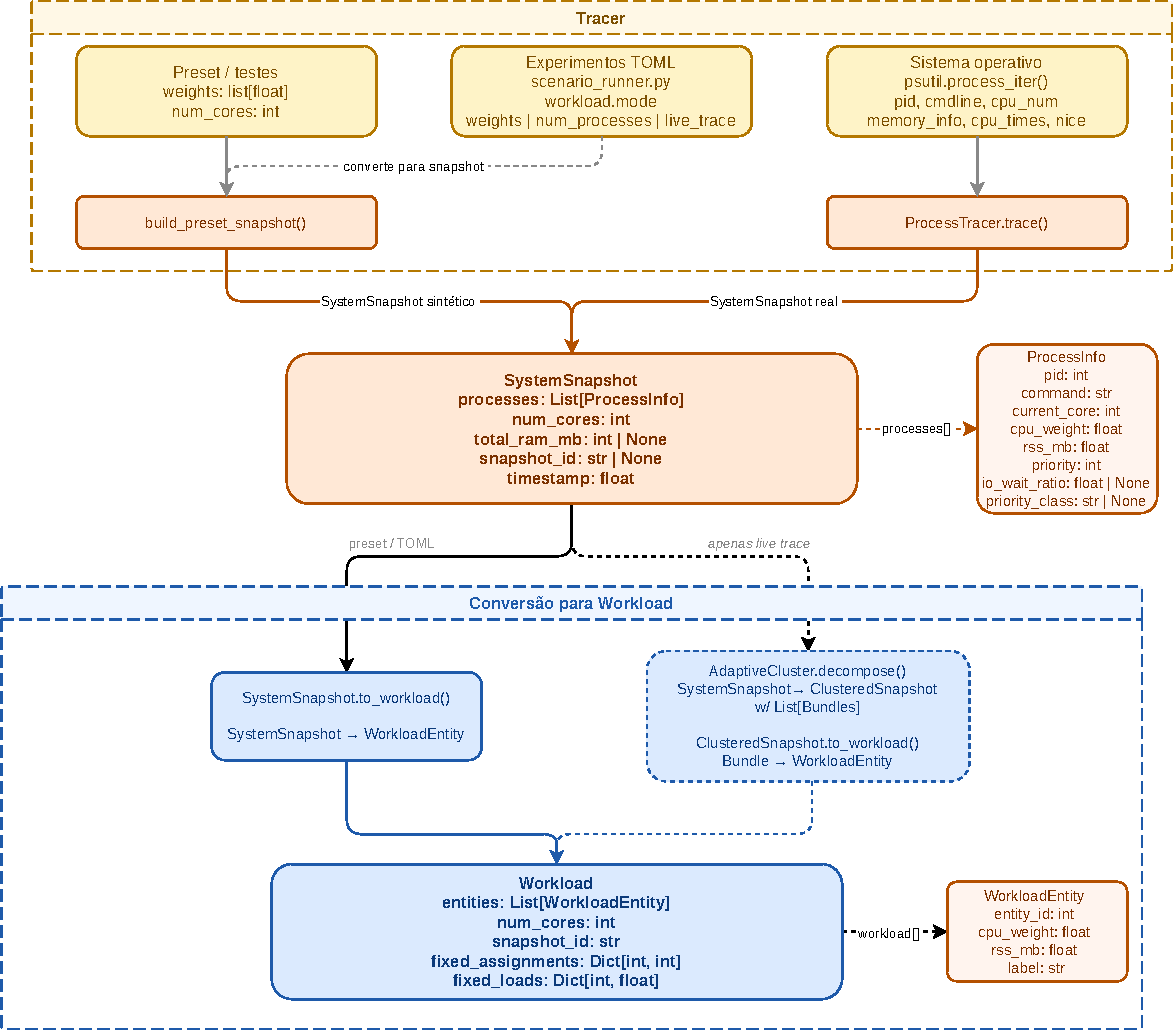
\includegraphics[width=\textwidth,height=\textheight,keepaspectratio]{images/diagrams/convergencia-systemsnapshot/data_contracts.pdf}
\caption{Interfaces de dados entre aquisição, \texttt{SystemSnapshot} e \texttt{Workload}.}
\label{fig:data-contracts}
\end{figure}

É neste ponto que a decisão $N \times K \leq q_{max}$ da visão geral aparece no
código, originando dois modos de execução:

\begin{itemize}
    \item se o limite de qubits permitir, a \texttt{DefaultPipeline} constrói uma
    \texttt{QUBOInstance} única através do \texttt{CoreAssignmentBuilder} e
    resolve-a diretamente;

    \item se o limite de qubits for excedido, é executada a
    \texttt{IterativePipeline}. Neste modo, é construída uma \texttt{QUBOInstance}
    global e o \texttt{SubQUBODecomposer} particiona o problema, extraindo em cada
    iteração uma nova \texttt{QUBOInstance} correspondente a um sub-QUBO.
\end{itemize}

Assim, as duas pipelines preservam a estrutura de dados que o \textit{solver}
espera receber.

A partir daqui, as \texttt{QUBOInstance} são entregues a um dos \textit{solvers}:

\begin{itemize}
    \item o \textit{solver} PennyLane implementa o \acs{QAOA};
    \item o \textit{solver} de \textit{annealing} serve como referência heurística;
    \item o brute-force fornece uma referência exata para instâncias pequenas.
\end{itemize}

Como todos usam a mesma entrada e devolvem o mesmo tipo de resultado,
\textit{SolverResult}, podem ser comparados facilmente.

Por fim, o \texttt{SolverValidator} recebe um \textit{SolverResult} e avalia a solução candidata.

A saída final distingue os dois caminhos:

\begin{itemize}
    \item \texttt{SchedulingOutput}, no caso direto;
    \item \texttt{IterativeSchedulingOutput}, no caso iterativo.
\end{itemize}

Em execuções experimentais, estes objetos são ainda serializados em ficheiros
\texttt{JSON}, \texttt{.txt}, métricas e figuras.

Por fim, a validação: a solução produzida
pelo \textit{solver} é descodificada e verificada antes de ser convertida em
métricas e ficheiros de saída.

\clearpage

\begin{figure}[H]
\centering
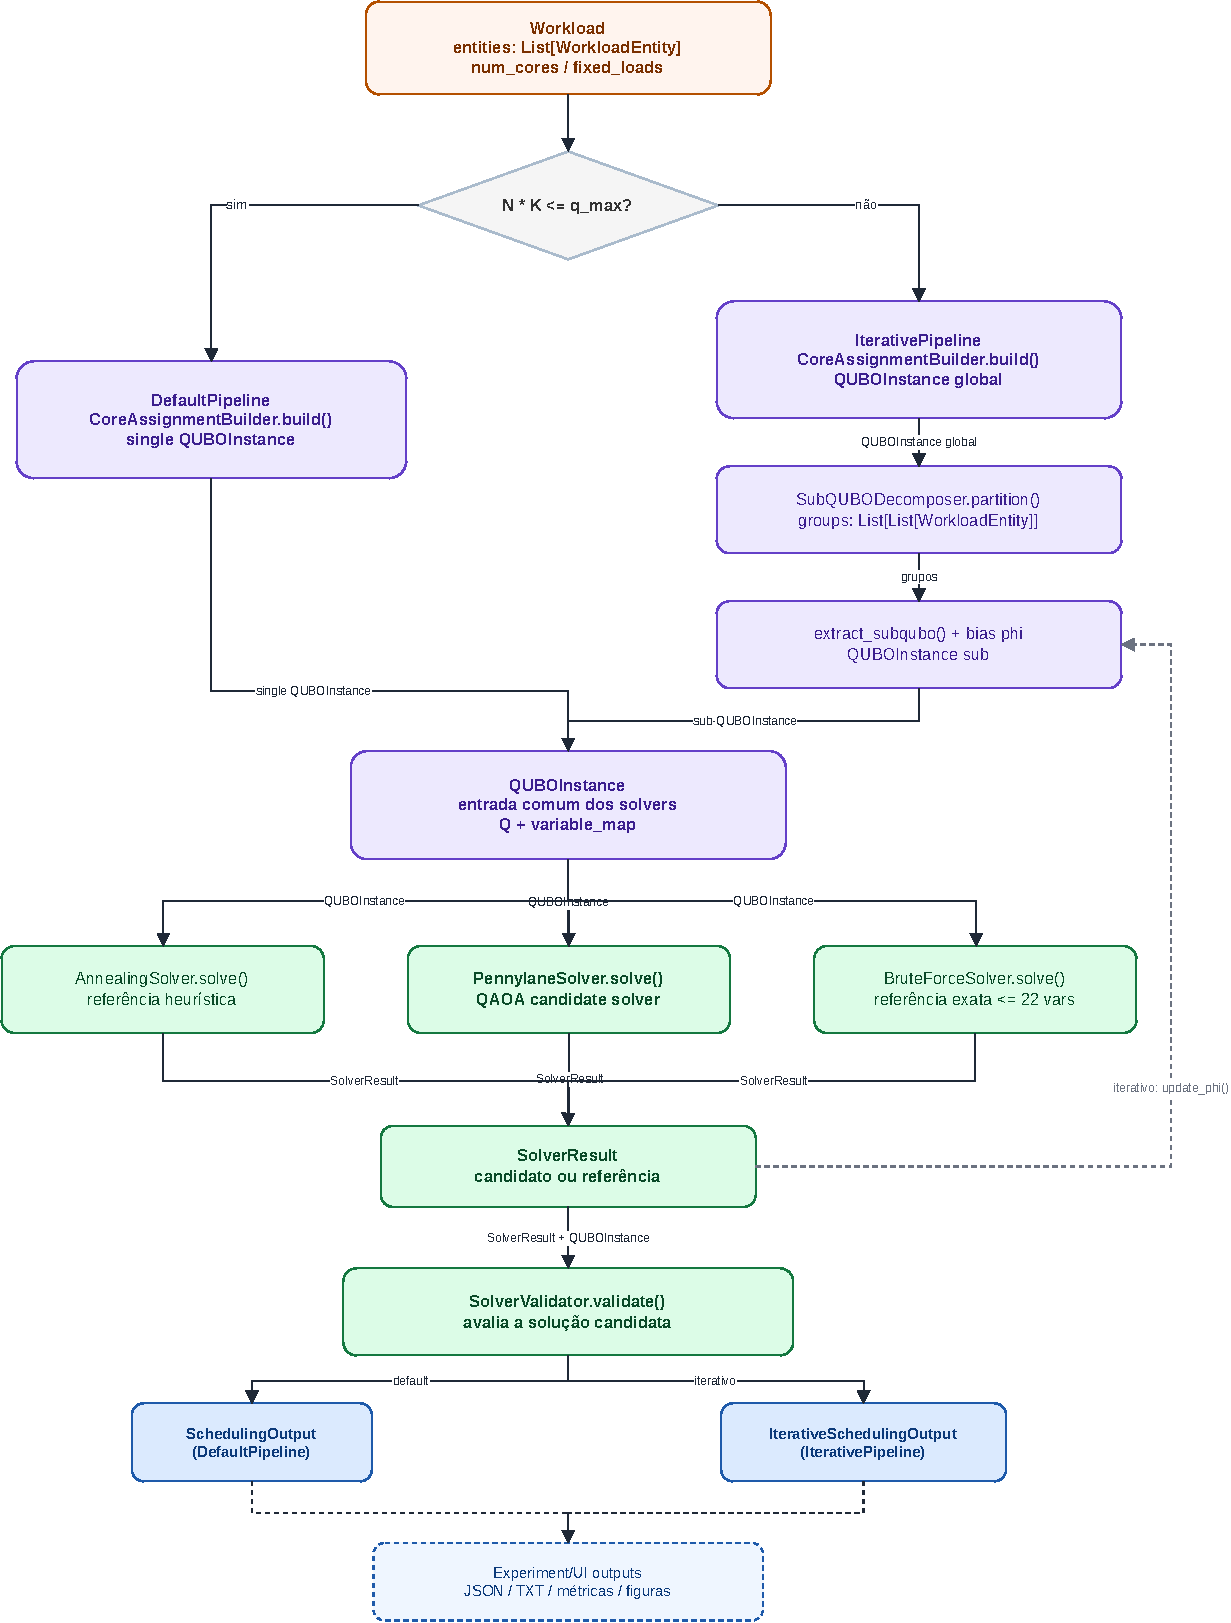
\includegraphics[width=\textwidth,height=\textheight,keepaspectratio]{images/diagrams/implementacao-arquitetura/implementacao-arquitetura.pdf}
\caption{Fluxo final de construção, resolução e validação das \texttt{QUBOInstance}.}
\label{fig:arquitetura-implementacao}
\end{figure}



\clearpage
\section{Estrutura do Projeto}
\label{sec:organizacao-projeto}

A implementação foi organizada de forma a refletir as principais etapas da
arquitetura. A diretoria \texttt{src/} contém o código principal do sistema,
separado por módulos, enquanto os testes e cenários experimentais são mantidos em diretorias próprias.

\begin{table}[H]
\centering
\small
\begin{tabular}{p{0.34\textwidth}p{0.58\textwidth}}
\hline
\textbf{Diretoria/Ficheiro} & \textbf{Função} \\
\hline
\texttt{src/main.py} & Define \texttt{SchedulingEngine} e a execução por linha de comandos. \\
\texttt{src/data\_contracts.py} & Centraliza as dataclasses e configurações partilhadas. \\
\texttt{src/builder/} & Constrói as matrizes \acs{QUBO}. \\
\texttt{src/solver/} & Implementa os \textit{solvers} e a validação das soluções. \\
\texttt{src/pipeline/} & Liga os módulos de construção, resolução e decomposição. \\
\texttt{src/decomposition/} & Agrupa snapshots reais e extrai \textit{sub-QUBOs}. \\
\texttt{src/tracer/} & Recolhe processos reais do sistema. \\
\texttt{src/visualizer/} & Gera visualizações e tabelas de diagnóstico. \\
\texttt{src/experiments/} & Define e executa cenários experimentais. \\
\hline
\end{tabular}
\caption{Mapa resumido da implementação.}
\label{tab:mapa-implementacao}
\end{table}

\subsection{Interfaces de Dados}
\label{subsec:interfaces-dados}

As interfaces de dados definidas em \texttt{data\_contracts.py} estabelecem a ligação
entre os módulos da implementação. Cada etapa da arquitetura recebe uma
estrutura de dados explícita, transforma-a e entrega uma nova interface à etapa
seguinte. Esta escolha torna o fluxo mais previsível e evita que os módulos
dependam diretamente dos detalhes internos uns dos outros.

\begin{table}[H]
\centering
\small
\begin{tabular}{p{0.40\textwidth}p{0.52\textwidth}}
\hline
\textbf{Interface} & \textbf{Papel na implementação} \\
\hline
\texttt{ProcessInfo} & Processo real capturado pelo tracer. \\
\texttt{SystemSnapshot} & Estado observado do sistema. \\
\texttt{WorkloadEntity} & Unidade abstrata a escalonar. \\
\texttt{Workload} & Problema de escalonamento entregue ao builder. \\
\texttt{ClusteredSnapshot} & Snapshot compactado após \textit{clustering}. \\
\texttt{QUBOInstance} & Formulação \acs{QUBO} entregue ao \textit{solver}. \\
\texttt{SolverResult} & Resposta normalizada de um \textit{solver}. \\
\texttt{SchedulingOutput} & Resultado final da pipeline direta. \\
\texttt{IterativeSchedulingOutput} & Resultado final da pipeline iterativa. \\
\hline
\end{tabular}
\caption{Interfaces de dados centrais.}
\label{tab:interfaces-dados}
\end{table}

Como exemplo, a interface \texttt{WorkloadEntity} representa uma unidade abstrata a
escalonar, independentemente de esta corresponder a um processo individual ou a um
\textit{bundle}. A sua definição reúne apenas os dados necessários às etapas seguintes:

\begin{lstlisting}[language=Python,caption={Exemplo da interface de dados \texttt{WorkloadEntity}.}]
@dataclass
class WorkloadEntity:
    entity_id: int
    cpu_weight: float
    rss_mb: float
    label: str
\end{lstlisting}

\subsection{Configurações}
\label{subsec:configuracoes}

Para além das interfaces de dados, a implementação separa os parâmetros de
execução em objetos de configuração. Alguns módulos e algoritmos dependem de
parâmetros ajustáveis, como limites de qubits, penalizações, critérios de decomposição entre outros. 

Para manter a modularidade e reduzir o
acoplamento entre componentes, estes parâmetros são agrupados em configurações
explícitas. Desta forma, é possível alterar o comportamento da pipeline sem
modificar a estrutura dos dados que circulam entre módulos.

\begin{table}[H]
\centering
\small
\begin{tabular}{p{0.40\textwidth}p{0.52\textwidth}}
\hline
\textbf{Configuração} & \textbf{Papel na implementação} \\
\hline
\texttt{QUBOConfig} & Define os parâmetros usados na construção da formulação \acs{QUBO}. \\
\texttt{QAOAConfig} & Controla a execução do \acs{QAOA}, incluindo camadas, passos, aprendizagem e tipo de mixer. \\
\texttt{TracerConfig} & Configura a recolha de processos reais pelo tracer. \\
\texttt{DecompositorConfig} & Define os limites e heurísticas usados na decomposição adaptativa. \\
\hline
\end{tabular}
\caption{Configurações principais da implementação.}
\label{tab:configuracoes}
\end{table}

\section{Conclusão}
\label{sec:arquitetura-sintese}

A arquitetura implementada foi pensada principalmente para reduzir acoplamento entre módulos.
Como consequência, novas fontes de workload, novos \textit{solvers} ou novas
estratégias de decomposição podem ser introduzidos sem alterar a estrutura
global da pipeline. Esta característica torna a plataforma adequada enquanto
\textit{testbed} para investigação e comparação de abordagens.
